\section{előadás (2025. november 4.)}
% Optimális zárójelezés (5. pont) folytatása

Ha az $l[i,j]$ értékek mellett feljegyezzük az optimumot adó $k$ értékeket is egy $k[i, j]$ táblázatban, akkor egy $k[1, n]$ fogja megmutatni az utolsó szorzást, pl. 9 mátrix esetén ha $k[1, 9] = 6$, akkor az optimális zárójelezés úgy néz ki, hogy
\begin{flalign*}
    &\underbrace{(A_1 A_2 \cdots A_6)}_{\text{ezek is zárójelezve vannak}} \underbrace{(A_7 A_8 A_9)}_{\text{ezek is}} &&
\end{flalign*}

Hogyan?
Általánosan:
\begin{flalign*}
    &\underbrace{(A_1 \cdots A_{k[1, n]})}_{\text{itt az első szorzás helyét ($k[1, k[1, n]]$)}} \underbrace{(A_7 A_8 A_9)}_{\text{itt pedig $k[k[1, n] + 1, n]$ helyét mutatja}} &&\\
\end{flalign*}

Az előző példát ha nézzük és azt mondjuk $k[1, 6] = 3$ és $k[1, 9] = 8$, akkor a zárójelezés egy szintet lejjebb lépve $((A_1 A_2 A_3)(A_4 A_5 A_6))((A_7 A_8) A_9)$ és így tovább.

\subsection{Sztringológia}
String-ekkel, string-ek hasonlóságával kapcsolatos kérdésekre keresünk válaszokat (gyorsan).

\subsubsection*{Az egyik legegyszerűbb ilyen kérdés}
Egy adott $T$ karaktersorozat tartalmaz-e egy adott $P$ karaktersorozatot?

Híres algoritmus: (Knuth-Morris-Pratt) $\rightarrow \Theta(|T| + |P|)$ ($|T|$ és $|P|$ a string-ek hossza)
Fő ötlet $P$ előfeldolgozása (Dinamikus Programozás).

\subsubsection*{Egy másik kérdés}
Adott egy $X$ és egy $Y$ karaktersorozat.
Keressük a leghosszabb közös részsorozatokat.
\begin{flalign*}
    & X = (x_1, x_2, \cdots, x_m) &&\\
    & Y = (y_1, y_2, \cdots, y_n) &&
\end{flalign*}

Ezeknek $Z = (z_1, z_2, \cdots, z_k)$ egy közös részsorozata lesz, ha léteznek olyan 
\begin{flalign*}
    & 1 \leq i_1 < i_2 < \cdots < i_k \leq m &&\\
    & 1 \leq j_1 < j_2 < \cdots < j_k \leq n &&
\end{flalign*}
részsorozatok, hogy
\begin{flalign*}
    & x_{i_1} = y_{j_1} = z_1 &&\\
    & x_{i_2} = y_{j_2} = z_2 &&\\
    & \cdots &&\\
    & x_{i_k} = y_{j_k} = z_k &&
\end{flalign*}

Kérdés a legnagyobb ilyen $k$.
$X$ és $Y$ hasonló, ha ez a $k$ nagy, és különböző, ha kicsi.

Például:
\begin{flalign*}
    & X = \text{\fbox{A}C\fbox{G}\fbox{C}T\fbox{A}G\fbox{C}} &&\\
    & Y =  \text{\fbox{A}T\fbox{G}\fbox{C}\fbox{A}ATC\fbox{C}} &&\\
    & Z =  \text{AGCAC} &&\\
\end{flalign*}

\subsubsection*{Egy harmadik}
Megint kiindulunk egy $X$ és egy $Y$ karaktersorozatból, de a hasonlóság definíciója kicsit más lesz.

Legyen $X = (x_1, x_2, \cdots, x_m)$ és $Y = (y_1, y_2, \cdots, y_n)$.
Az $X$ és $Y$ között bevezetjük a szekvenciaáttekintés fogalmát: ez egy párosítás az $X$-beli pozíciók és az $Y$-beli pozíciók között:
$M \subseteq \left\{ 1, 2, \cdots, m \right\} \times \left\{ 1, 2, \cdots, n \right\}$,
úgy, hogy minden $X$-beli és minden $Y$-beli legfeljebb egy $M$-beli párban fordul elő (kimaradhat pár pozíció)
ÉS ha $(i, j), (i', j') \in M$ és $i \leq i'$, akkor $j \leq j'$.

Például:

\begin{tabular}{l l l l l l l l}
    X = & A & C & G & A & C & G & T \\
        & 1 & 2 & 3 & 4 & 5 & 6 & 7
\end{tabular}

\begin{tabular}{l l l l l l l l l}
    Y = &C&A&G&A&T&G&G&A \\
        &1&2&3&4&5&6&7&8
\end{tabular}

Az $M$ szekvenciaillesztés itt lehet pl. $M = \left\{ (1, 2), (3, 3), (4, 4), (5, 6), (6, 7) \right\}$.

Vizuálisan (pozíciókat nézve):\\
\begin{tikzpicture}[
    roundnode/.style={circle, draw=black, minimum size=0.3cm, inner sep=0.5mm}
]
\node[roundnode](t1){$1$};
\node[roundnode](t2)[right = 0.4cm of t1]{$2$};
\node[roundnode](t3)[right = 0.4cm of t2]{$3$};
\node[roundnode](t4)[right = 0.4cm of t3]{$4$};
\node[roundnode](t5)[right = 0.4cm of t4]{$5$};
\node[roundnode](t6)[right = 0.4cm of t5]{$6$};
\node[roundnode](t7)[right = 0.4cm of t6]{$7$};

\node[roundnode](l1)[below = 0.4cm of t1]{$1$};
\node[roundnode](l2)[right = 0.4cm of l1]{$2$};
\node[roundnode](l3)[right = 0.4cm of l2]{$3$};
\node[roundnode](l4)[right = 0.4cm of l3]{$4$};
\node[roundnode](l5)[right = 0.4cm of l4]{$5$};
\node[roundnode](l6)[right = 0.4cm of l5]{$6$};
\node[roundnode](l7)[right = 0.4cm of l6]{$7$};
\node[roundnode](l8)[right = 0.4cm of l7]{$8$};

\draw (t1) -- (l2);
\draw (t3) -- (l3);
\draw (t4) -- (l4);
\draw (t5) -- (l6);
\draw (t6) -- (l7);
\end{tikzpicture}


Az $i < i'$ feltétel kizárja pl. a következőt:
\begin{tikzpicture}[
    roundnode/.style={circle, draw=black, minimum size=0.3cm, inner sep=0.5mm}
]
\node[roundnode](l5){$5$};
\node[roundnode](t7)[above right = 0.4cm and 1.1cm of l5]{$7$};

\draw (l5) -- (t7);
\end{tikzpicture}


A szekvenciaillesztés megjeleníthető az $X$ karaktersorozatból az $Y$ karaktersorozat előállításaként karakterek törlése, beszúrása, cseréje (változatlanul hagyása) egymásutánjaként.

Az előző példában minden ferde vonalat függőlegessé teszünk:\\
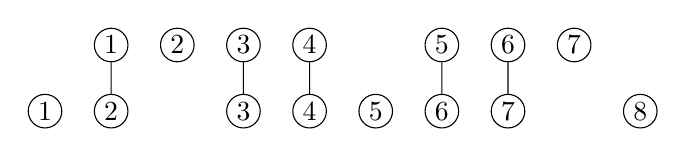
\begin{tikzpicture}[
    scale=0.84,
    roundnode/.style={circle, draw=black, minimum size=0.3cm, inner sep=0.5mm}
]
\node[roundnode](t1) at (1, 1) {$1$};
\node[roundnode](t2) at (2, 1) {$2$};
\node[roundnode](t3) at (3, 1) {$3$};
\node[roundnode](t4) at (4, 1) {$4$};
\node[roundnode](t5) at (6, 1) {$5$};
\node[roundnode](t6) at (7, 1) {$6$};
\node[roundnode](t7) at (8, 1) {$7$};

\node[roundnode](l1) at (0, 0) {$1$};
\node[roundnode](l2) at (1, 0) {$2$};
\node[roundnode](l3) at (3, 0) {$3$};
\node[roundnode](l4) at (4, 0) {$4$};
\node[roundnode](l5) at (5, 0) {$5$};
\node[roundnode](l6) at (6, 0) {$6$};
\node[roundnode](l7) at (7, 0) {$7$};
\node[roundnode](l8) at (9, 0) {$8$};

\draw (t1) -- (l2);
\draw (t3) -- (l3);
\draw (t4) -- (l4);
\draw (t5) -- (l6);
\draw (t6) -- (l7);
\end{tikzpicture}

Nézzük a betűket:

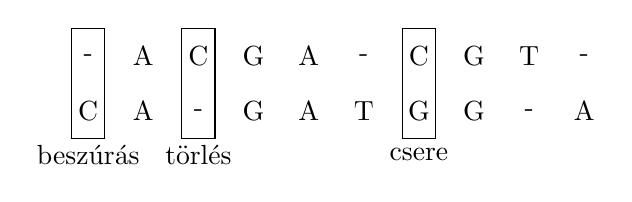
\begin{tikzpicture}[scale=0.7]
\node(t1) at (1, 1) {-};
\node(t2) at (2, 1) {A};
\node(t3) at (3, 1) {C};
\node(t4) at (4, 1) {G};
\node(t5) at (5, 1) {A};
\node(t6) at (6, 1) {-};
\node(t7) at (7, 1) {C};
\node(t8) at (8, 1) {G};
\node(t9) at (9, 1) {T};
\node(t10) at (10, 1) {-};

\node(l1) at (1, 0) {C};
\node(l2) at (2, 0) {A};
\node(l3) at (3, 0) {-};
\node(l4) at (4, 0) {G};
\node(l5) at (5, 0) {A};
\node(l6) at (6, 0) {T};
\node(l7) at (7, 0) {G};
\node(l8) at (8, 0) {G};
\node(l9) at (9, 0) {-};
\node(l10) at (10, 0) {A};

\draw (0.7,-0.5) rectangle ++(0.6,2);
\node at (1,-0.8) {beszúrás};
\draw (2.7,-0.5) rectangle ++(0.6,2);
\node at (3,-0.8) {törlés};
\draw (6.7,-0.5) rectangle ++(0.6,2);
\node at (7,-0.8) {csere};
\end{tikzpicture}

Az $X$ transzformációja $Y$-ná ennek megfelelően:
\begin{enumerate}
    \item Szúrjunk be egy C-t
    \item Másoljuk A-t
    \item Töröljük C-t
    \item Másoljuk G-t
    \item Másoljuk A-t
    \item Szúrjunk be egy T-t
    \item Cseréljük C-t G-re
    \item $\cdots$
\end{enumerate}

Persze nem csak ez az egy lehetőség van.
Melyiket használjuk a hasonlóság mérésére?

Egy $M$ szekvenciaillesztés minőségét a következőképpen definiáljuk:
\begin{enumerate}
    \item az $M$-ben nem szereplő pozíciókra felszámolunk egy fix $y > 0$ értéket (ez része az inputnak)
    \item ha $(i, j) \in M$, akkor erre felszámolunk egy $c["p", "q"] \geq 0$ értéket, ahol $x_i = "p"$ és $y_j = "q"$ (ez is része az inputnak)
\end{enumerate}

Ezeket összeadjuk, és keressük a legjobb minőségű szekvenciaillesztést, vagyis egy olyat, ahol ez az összeg minimális.

Az összes szekvenciaillesztés végigbogarászása exponenciálisan hosszú idő: $DP \rightarrow \Theta(mn)$.
Erős érvek szólnak amellett, hogy ennél polinomiálisan hatékonyabb algoritmus nem létezik.

[megjegyzés: $\theta(\frac{mn}{\log m+n})$ aszimptotikusan hatékonyabb, de polinomiálisan nem]

\subsubsection*{DP algoritmus}
Miféle részproblémák jöhetnek elő itt?
Az eddigi szerény tapasztalataink alapján: 
optimális szekvenciaillesztés $(x_i, x_{i+1}, \cdots, x_j)$, $(y_k, y_{k+1}, \cdots, y_l)$ között (infixek).

Kiderül, hogy prefixek is elegek lesznek.
$R[i, j]$ részprobléma: $(X_i) = (x_1, x_2, \cdots, x_i)$ és $(Y_j) = (y_1, y_2, \cdots, y_j)$ optimális szekvenciaillesztés meghatározása.













